\documentclass[11pt, a4paper]{article}
\usepackage[margin=2.4cm]{geometry}
\usepackage[T1]{fontenc}
\usepackage{lmodern}          % Type 1 vector fonts
\usepackage{cmap}             % ToUnicode CMap -> copyable text and accents
\usepackage[utf8]{inputenc}
\usepackage[english]{babel}
\usepackage{amsmath, amssymb, amsthm}
\usepackage{bm}
\usepackage{mathtools}
\usepackage{enumitem}
\usepackage{booktabs}
\usepackage{array}
\usepackage{xcolor}
\usepackage{titlesec}
\usepackage{parskip}
\usepackage{hyperref}
\usepackage{fancyhdr}
\usepackage{tcolorbox}
\usepackage{graphicx}
\usepackage{caption}
\tcbuselibrary{skins, breakable}

\definecolor{darkblue}{RGB}{15,55,115}
\definecolor{midblue}{RGB}{30,100,180}
\definecolor{theorybg}{RGB}{245,250,255}
\definecolor{questionbg}{RGB}{255,252,240}
\definecolor{evencolor}{RGB}{60,0,100}
\definecolor{rubricbg}{RGB}{248,246,252}
\definecolor{planbg}{RGB}{246,252,247}
\definecolor{plancolor}{RGB}{20,95,55}
\definecolor{trapbg}{RGB}{255,247,245}
\definecolor{trapcolor}{RGB}{150,35,35}

\hypersetup{colorlinks=true, linkcolor=darkblue, urlcolor=midblue,
  pdftitle={Solutions --- Problem Set 7 --- Macroeconomics I MPE Insper},
  pdfauthor={Macroeconomia I --- MPE Insper 2026/T3}}

\setlength{\headheight}{14pt}
\pagestyle{fancy}
\fancyhf{}
\renewcommand{\headrulewidth}{0.4pt}
\fancyhead[L]{\small\textcolor{darkblue}{\textit{Macroeconomia I --- MPE Insper --- 2026/T3}}}
\fancyhead[R]{\small\textcolor{darkblue}{\thepage}}
\fancyfoot[C]{\small\textcolor{gray}{Solutions --- Problem Set 7}}

\titleformat{\section}[block]
  {\large\bfseries\color{darkblue}}{}{0pt}{}
  [\vspace{2pt}\color{darkblue}\rule{\textwidth}{1.5pt}\vspace{4pt}]

\tcbset{
  theorybox/.style={
    enhanced, breakable, colback=theorybg, colframe=darkblue,
    fonttitle=\bfseries\small, coltitle=white, boxrule=0.5pt, arc=3pt,
    left=6pt, right=6pt, top=4pt, bottom=4pt,
  },
  questionbox/.style={
    enhanced, breakable, colback=questionbg, colframe=gray!60,
    fonttitle=\bfseries\small, coltitle=black, boxrule=0.4pt, arc=2pt,
    left=6pt, right=6pt, top=4pt, bottom=4pt, title={\textit{Question}},
  },
  rubricbox/.style={
    enhanced, breakable, colback=rubricbg, colframe=evencolor!70,
    fonttitle=\bfseries\small, coltitle=white, boxrule=0.4pt, arc=2pt,
    left=6pt, right=6pt, top=4pt, bottom=4pt, title={Where the marks are},
  },
  planbox/.style={
    enhanced, breakable, colback=planbg, colframe=plancolor,
    fonttitle=\bfseries\small, coltitle=white, boxrule=0.5pt, arc=3pt,
    left=6pt, right=6pt, top=4pt, bottom=4pt,
  },
  trapbox/.style={
    enhanced, breakable, colback=trapbg, colframe=trapcolor!75,
    fonttitle=\bfseries\small, coltitle=white, boxrule=0.4pt, arc=2pt,
    left=6pt, right=6pt, top=4pt, bottom=4pt,
  },
}

\newcommand{\passo}[1]{\medskip\noindent\textbf{#1}\par\nobreak}
\newcommand{\intuicao}[1]{%
  \medskip\noindent\textcolor{midblue}{\textbf{Economic reading.}} #1\par}
\newcommand{\resp}[1]{%
  \ifmmode {\color{darkblue}#1}\else\textcolor{darkblue}{\textbf{#1}}\fi}
\newcommand{\stst}{^{\ast}}
\newcommand{\MRS}{\mathrm{MRS}}
\newcommand{\MRT}{\mathrm{MRT}}

\setlist[enumerate,1]{label=(\alph*), itemsep=6pt, parsep=2pt, leftmargin=1.6em}
\setlist[itemize,1]{itemsep=3pt, parsep=1pt, leftmargin=1.3em, topsep=3pt}

\newcommand{\ybn}{\bar y_n}
\newcommand{\pbar}{\bar p}
\newcommand{\Sg}{\left(\sigma^{-1}+\eta\right)}
% Companion links: local files, and the published private copies.
\newcommand{\compdir}{../Map/benigno}
\newcommand{\urlshocks}{https://claude.ai/artifact/Hf8KsQYWvTwd6BnyFXP7MZ}
\newcommand{\urlwedge}{https://claude.ai/artifact/KUhe4SoMSCrZb5z7afiJ9U}
\newcommand{\urlloss}{https://claude.ai/artifact/5LYyfukdcNiBd3cHXvWH63}
\newcommand{\urlthree}{\compdir/companion-as-ad.html}

\begin{document}

%======================================================================
\begin{center}
{\LARGE\bfseries\color{darkblue} Solutions --- Problem Set 7\par}
\vspace{4pt}
{\large MACROECONOMIA 1 --- MPE Insper --- Prof.\ Pedro G.\ Duarte\par}
\vspace{2pt}
{\normalsize 2026, 3\textordmasculine{} trimestre \quad$\cdot$\quad Due: 25/09\par}
\vspace{2pt}
{\small The New-Keynesian AS--AD model --- Benigno (2015), \S\S1--12\par}
\end{center}
\vspace{6pt}

\begin{tcolorbox}[theorybox, title={How to read this document}]
\small
This file answers \textbf{all four questions} (10 points). No textbook exercise sits behind
this list: every item is built on Benigno (2015), ``New-Keynesian economics: an AS--AD
view'', \emph{Research in Economics} 69, printed pages 503--524, which is the reading for
lectures 8 and 9.

\smallskip
\textbf{The thread.} The four questions are one argument told four times.
Question 1 asks \emph{why} the New-Keynesian model has the ingredients it has. Question 2 uses
them: one shock that moves AS, one policy that moves AD. Question 3 isolates the single
ingredient --- the mark-up wedge --- that makes the natural and the efficient level of output
different objects. Question 4 shows what a central bank does once they are different: it
minimises a welfare loss, and the AS curve is the menu it must choose from.

\smallskip
\textbf{The model, once.} Every answer below uses only these lines (Benigno's notation:
lower-case letters are log-deviations from an efficient steady state):
\begin{align*}
\text{AS (17), (20):}\quad & p-p^e=\kappa\,(y-y_n),\qquad
  \kappa\equiv\frac{(1-\alpha)\Sg}{\alpha},\\
\text{AD (21):}\quad & y=\ybn+(g-\bar g)-\sigma\left[i-(\pbar-p)-(\bar\tau_c-\tau_c)-\rho\right],\\
\text{natural (15):}\quad & y_n=\frac{(1+\eta)a+\sigma^{-1}g-\mu}{\sigma^{-1}+\eta},
\qquad\text{efficient (19):}\quad y_e=\frac{(1+\eta)a+\sigma^{-1}g}{\sigma^{-1}+\eta}.
\end{align*}
Numbers use Benigno's own calibration: $\alpha=0.66$, $\sigma=0.5$, $\eta=0.2$ (p.~515), so
$\kappa=1.133$; and $\theta=8$ (fn.~24, p.~522). They are computed in
\texttt{Resolucao/lista7\_codigo/l7\_figuras.py}, which prints every figure quoted here.

\smallskip
\textbf{Companions.} Three interactive pages were built for this list. Each has its own
controls and its read-outs are the closed forms below, evaluated live:
\href{\urlshocks}{\emph{Two Shocks}} (Q2), \href{\urlwedge}{\emph{The Wedge}} (Q3),
\href{\urlloss}{\emph{The Loss Bowl}} (Q4). Local copies are in \texttt{Map/benigno/}.
The full derivation of every equation is in the note set \texttt{Map/benigno/00-index.md}.

\smallskip
Highlighted answers are in \resp{blue}. \textcolor{trapcolor}{\textbf{Red}} boxes are traps;
\textcolor{plancolor}{\textbf{green}} boxes are method. \emph{Language:} English, per the
project's global output rule; the problem set is itself in English.
\end{tcolorbox}

\begin{center}
\small
\begin{tabular}{@{}lcl@{}}
\toprule
\textbf{Item} & \textbf{Points} & \textbf{Basis in Benigno (2015)} \\
\midrule
1 --- NK vs New Classical vs Keynesian & 3 & \S1--\S4, \S11; pp.\ 503--508, 521--522 \\
2(a) --- temporary mark-up rise & 1.5 & \S7, Fig.\ 9, pp.\ 513--514 \\
2(b) --- nominal-rate cut & 1.5 & \S5, Figs.\ 3--5, pp.\ 509--511 \\
3 --- $y_n$ vs $y_e$ & 2 & \S4.1--\S4.4, eqs.\ (14), (15), (19), pp.\ 507--509 \\
4 --- the loss function and the AS constraint & 2 & \S11, eqs.\ (33)--(35), Fig.\ 14, pp.\ 521--523 \\
\bottomrule
\end{tabular}
\end{center}

%======================================================================
\section{Question 1 \quad Three generations of short-run macroeconomics}
%======================================================================

\begin{tcolorbox}[planbox, title={The one-sentence answer, before the table}]
\small
The New-Keynesian (NK) model takes its \textbf{method} from the New Classicals (optimising
agents, rational expectations, general equilibrium) and its \textbf{frictions} from the
Keynesians (nominal prices that do not clear markets in the short run). Two ingredients
turn that combination into a working model: \textbf{monopolistic competition}, so that
someone \emph{sets} the prices that are sticky, and an \textbf{interest-rate instrument},
so that demand is driven by the real rate through the Euler equation. Benigno (p.~503)
describes it as a model that keeps ``the classical dichotomy'' in the long run, while in
the short run ``monetary policy is not neutral, owing to the assumption of price
rigidity'' (p.~505).
\end{tcolorbox}

\begin{center}
\small
\renewcommand{\arraystretch}{1.25}
\begin{tabular}{@{}>{\raggedright\arraybackslash}p{2.1cm}
                >{\raggedright\arraybackslash}p{4.2cm}
                >{\raggedright\arraybackslash}p{4.2cm}
                >{\raggedright\arraybackslash}p{4.3cm}@{}}
\toprule
& \textbf{Original Keynesian} (IS--LM + Phillips curve, 1950s--60s)
& \textbf{New Classical} (Lucas, Sargent--Wallace, Barro, 1970s)
& \textbf{New Keynesian} (1980s on; Benigno 2015) \\
\midrule
(i) Prices, expectations, money
& Wages/prices rigid by assumption; expectations adaptive or absent; a stable, exploitable
  Phillips curve; money has lasting real effects.
& Prices and wages flexible, markets clear; rational expectations; only \emph{unanticipated}
  money moves output (misperceptions); systematic policy is ineffective.
& Rational expectations \emph{plus} pre-set prices: a fraction $\alpha$ keeps $p^e$.
  Policy that reacts after $p^e$ is set moves output even if fully anticipated; neutral in
  the long run. \\
(ii) Market structure
& Unmodelled or competitive; price level set by a rule of thumb or a rigid nominal wage.
& Perfect competition: price-takers, no one sets a price.
& Monopolistic competition (Dixit--Stiglitz): firms set $P(j)=(1+\mu)W/A$, so $P>$ marginal
  cost and firms serve extra demand at a fixed price. \\
(iii) AD and the instrument
& IS from a consumption function, LM from money demand; the central bank sets $M$; AD
  slopes down through real balances.
& Demand is the quantity equation $MV=PY$; money supply is the instrument and the source
  of nominal shocks.
& AD is the Euler equation; no LM curve; the central bank sets $i$; AD slopes down because
  a higher $p$ with $\pbar$ fixed raises the real rate. \\
(iv) Micro-foundations and welfare
& Behavioural equations postulated and estimated; policy judged by an ad hoc loss.
& Full micro-foundations; equilibrium is efficient, so there is nothing for stabilisation
  policy to fix.
& Micro-founded \emph{and} distorted: the welfare loss is derived from utility,
  $\tfrac12(y-y_e)^2+\tfrac{\theta}{2\kappa}(p-p^e)^2$ (eq.\ 33). \\
\bottomrule
\end{tabular}
\end{center}

Each row is expanded below, in the order the question asks: \emph{what each school does},
\emph{the evidence that pushed the NK formulation}, and \emph{what it implies for the
structure and predictions of the model}.

%----------------------------------------------------------------------
\subsection*{(i) Price adjustment, expectations, and the short-run effects of monetary policy}
%----------------------------------------------------------------------

\passo{Original Keynesian.}
Nominal wages (in Keynes) or prices are rigid, and the rigidity is an \emph{assumption}. It is
not derived from anyone's choice. Expectations are either absent or adaptive, so the Phillips
curve of the 1960s is read as a stable menu: more inflation buys permanently less
unemployment. Monetary policy has real effects that last as long as the rigidity does.

\passo{New Classical.}
Prices and wages clear markets continuously, and expectations are rational. Money moves
output only through \emph{surprises}: in Lucas's imperfect-information model, a producer who
cannot tell a general price rise from a rise in the relative price of their own good supplies
more when the price level is unexpectedly high. That gives the ``New-Classical Phillips
curve'', $p-p^e=\kappa(y-y_n)$, of Phelps (1967) and Lucas (1973). Its policy implication is
the Sargent--Wallace \emph{policy-ineffectiveness proposition}: any systematic rule is built
into expectations, so only random policy moves output, and random policy is useless.

\passo{New Keynesian.}
Rational expectations stay. Price rigidity comes back, but now as a \emph{choice}. In Benigno
\S4 (p.~507) a fraction $\alpha$ of firms must keep the price $P^e$ they fixed \emph{before}
the shock is observed. Two justifications are given on that page. Under monopolistic
competition, a firm at its optimum loses only a \emph{second-order} amount from a small
price error, so a tiny menu cost (Mankiw, 1985) is enough to rationalise not adjusting. And
the same algebra describes \emph{sticky information}. Remarkably, the resulting AS curve has
exactly the New-Classical form:
\[
p-p^e=\kappa\,(y-y_n),\qquad \kappa=\frac{(1-\alpha)\Sg}{\alpha}.
\]
Benigno says so openly (p.~508): the equation is the one Phelps and Lucas derived, ``derived
on different principles''. What changes is the \emph{reading}:
\begin{itemize}
\item $p^e$ is not a forecast that might be wrong; it is a \emph{price already posted}. A
      central bank that responds to a shock \emph{after} $p^e$ is set moves output even if
      everybody knows its rule. That is the difference with policy ineffectiveness:
      \resp{systematic stabilisation policy works, because it acts faster than prices can.}
\item The slope is no longer a free parameter. $\kappa$ is built from the share of sticky
      firms $\alpha$ and the preference parameters $(\sigma,\eta)$. More rigidity means a
      \emph{flatter} AS curve, and in the limit $\alpha\to0$ the AS curve is vertical and the
      model is classical again.
\item In the long run every firm resets, the Phillips curve is vertical, and money is
      neutral: $\pbar$ appears nowhere in $\ybn$ (Benigno \S4.2, p.~508).
\end{itemize}

\passo{Empirical motivation.}
Three facts pushed the profession to this combination.
\begin{enumerate}[label=\arabic*.]
\item \emph{The 1970s.} Inflation and unemployment rose together, so the stable
      Keynesian Phillips curve broke down. That vindicated the New-Classical insistence that
      expectations adjust, and every NK model keeps rational expectations for this reason.
\item \emph{Monetary policy has large, persistent real effects} even when it is announced
      and data on money and prices are published within weeks. Pure misperception cannot
      last that long. The costly Volcker disinflation of 1979--82 is the standard example.
      This argues for a friction that does not depend on anyone being fooled.
\item \emph{Micro price data} show that individual prices are changed infrequently. Benigno
      calibrates an average price duration of about three quarters for the United States,
      i.e.\ $\alpha\simeq0.66$ (p.~515). That fact is what disciplines $\kappa$.
\end{enumerate}

\passo{Implications for the structure and the predictions.}
The model has a two-period structure with a \emph{non-vertical} short-run AS curve and a
\emph{vertical} long-run one. Its central prediction is short-run non-neutrality together
with long-run neutrality. The size of the real effect of policy is governed by
$\sigma\kappa$: from the closed-form solution,
$dy=-\sigma\,di/(1+\sigma\kappa)$. With rigid prices, $\kappa\to0$ and the rate cut goes
entirely into output; with flexible prices, $\kappa\to\infty$ and it goes entirely into
prices.

%----------------------------------------------------------------------
\subsection*{(ii) Market structure and firms' price-setting behaviour}
%----------------------------------------------------------------------

\passo{Original Keynesian.}
Market structure is left unmodelled. Where a price equation exists it is a mark-up rule of
thumb or follows from a rigid nominal wage with competitive firms. In the latter case the
real wage must be \emph{counter}-cyclical, since firms move along a falling marginal-product
curve.

\passo{New Classical.}
Perfect competition. Everybody takes prices as given, so the model contains no agent whose
decision \emph{is} the price. A theory of sticky prices has nobody to attach the stickiness
to.

\passo{New Keynesian.}
Monopolistic competition in the Dixit--Stiglitz form (Benigno eq.\ 9; Blanchard and
Kiyotaki, 1987). Firm $j$ faces demand $Y(j)=(P(j)/P)^{-\theta}(C+G)$, and profit
maximisation gives a constant mark-up over marginal cost (eq.\ 11):
\[
P(j)=\frac{\theta}{\theta-1}\cdot\frac{1+\tau_w}{1-\tau_y}\cdot\frac{W}{A}
\;=\;(1+\tilde\mu)\,\frac{W}{A}.
\]
Monopolistic competition does three separate jobs, and each is structural:
\begin{enumerate}[label=\arabic*.]
\item \textbf{Someone sets prices}, so a pre-set price $P^e$ is a well-defined decision.
\item \textbf{Price exceeds marginal cost}, so a firm stuck at $P^e$ is \emph{willing} to
      serve extra demand. Output in the short run is therefore \emph{demand-determined}, and
      that is why shifting AD moves $y$.
\item \textbf{The mark-up is a wedge.} It makes the natural level inefficiently low,
      $y_n<y_e$, and a change in the mark-up is an \emph{inefficient} shock. This is the
      entire content of Questions 3 and 4.
\end{enumerate}
It also explains why small frictions matter. The envelope theorem makes a firm's private
loss from not adjusting second order, while the aggregate effect on output is first order,
because output starts below its efficient level.

\passo{Empirical motivation.}
Firms visibly set and post prices and earn mark-ups. The real wage is not strongly
counter-cyclical, so a model in which all the rigidity sits in nominal wages with
competitive firms predicts the wrong co-movement. Putting rigidity in \emph{prices} set by
firms with market power fixes that.

\passo{Implications.}
The AS curve is a \emph{pricing} relation: only the $1-\alpha$ firms that can adjust move
their prices, in proportion to real marginal cost, which rises with $y-y_n$ (eq.\ 16). Its
anchor $(p^e,y_n)$ moves with anything that changes the mark-up: monopoly power, the taxes
$\tau_w,\tau_l,\tau_y,\tau_c$ in eq.\ (13), or an oil-price rise (p.~513). The model can
therefore talk about \emph{cost-push shocks}, which neither predecessor could.

%----------------------------------------------------------------------
\subsection*{(iii) The construction of aggregate demand and the monetary-policy instrument}
%----------------------------------------------------------------------

\passo{Original Keynesian.}
IS comes from a consumption function in \emph{current} income and investment in the
interest rate; LM comes from money demand; the central bank sets the money supply. AD slopes
down through real balances: a higher $P$ lowers $M/P$, raises $i$ and cuts investment.
Consumption does not depend on the future.

\passo{New Classical.}
Aggregate demand is essentially the quantity equation, with the money stock as the policy
variable and the source of nominal disturbances.

\passo{New Keynesian (Benigno \S3).}
AD is the household's \textbf{Euler equation} combined with the resource constraint:
\[
y=\ybn+(g-\bar g)-\sigma\left[i-(\pbar-p)-(\bar\tau_c-\tau_c)-\rho\right].
\]
\begin{itemize}
\item \textbf{No LM curve, no money stock.} The central bank sets the short-term nominal
      rate $i$ directly, and money is supplied elastically at that rate. Benigno (p.~504):
      the analysis ``is consistent with the modern central banking practice of targeting
      short-term nominal interest rates, not money supply aggregates''.
\item \textbf{The slope is intertemporal.} With $\pbar$ given, a higher $p$ today lowers
      expected inflation $\pbar-p$, raises the real rate, and households postpone
      consumption. Money demand plays no role in it.
\item \textbf{The future is in today's demand.} $\ybn$ and $\pbar$ enter directly: news
      about long-run income, or a promise about the long-run price level, shifts demand now.
      Benigno calls intertemporal decisions ``another novelty with respect to Keynesian
      models'' (p.~505).
\end{itemize}

\passo{Empirical motivation.}
Central banks set interest rates; they do not target monetary aggregates, and money
demand proved too unstable to make money targets reliable. The Euler-equation demand also
builds the Lucas critique in, since its parameters are preferences and not reduced-form
propensities.

\passo{Implications.}
Transmission runs through the \emph{real} rate. Policy works through \emph{expectations}
($\pbar$ enters AD exactly where $-i$ does; see Benigno \S9). The model can have a
\emph{zero lower bound}, because the instrument is a rate. And it predicts \emph{smaller}
fiscal multipliers in normal times than the Keynesian cross: a rise in $g$ has a multiplier
below one on output (Benigno \S8, p.~514).

%----------------------------------------------------------------------
\subsection*{(iv) Micro-foundations and welfare analysis}
%----------------------------------------------------------------------

\passo{Original Keynesian.}
Behavioural equations are postulated and estimated. Policy is judged by a loss function that
the modeller writes down. Its targets and weights express the analyst's preferences, not the
households'.

\passo{New Classical.}
Full micro-foundations, but in a frictionless competitive economy. By the First Welfare
Theorem the equilibrium is efficient, so fluctuations are optimal responses and there is
nothing for stabilisation policy to fix.

\passo{New Keynesian.}
Micro-foundations \emph{with} distortions: market power, taxes and sticky prices. Because the
model has a household utility function and identifiable distortions, the objective of policy
is \emph{derived}. A second-order approximation to utility around an efficient steady state
gives Benigno's eq.\ (33):
\[
L=\tfrac12\left(y-y_e\right)^2+\frac{\theta}{2\kappa}\left(p-p^e\right)^2 .
\]
This loss says three things no ad hoc loss can justify. The output target is the
\emph{efficient} level $y_e$, not the natural level. Only \emph{unanticipated} price
movements are costly, because with a share $\alpha$ of prices frozen they create
relative-price dispersion across identical goods. And the weight on prices, $\theta/\kappa$,
rises with rigidity and with substitutability. Welfare analysis then answers questions a
Keynesian model cannot even pose. Which shocks create a trade-off? Only mark-up shocks, as
Question 3 shows. Does a positive fiscal multiplier mean the policy is good? Not necessarily: Benigno
\S8 shows that a cut in the consumption tax raises output but has a \emph{negative} multiplier
on the output gap.

\passo{Empirical motivation.}
Large macro-econometric models broke down out of sample in the 1970s. The Lucas critique
says why: their coefficients shift when policy changes. Deep parameters $(\beta,\tilde\sigma,
\eta,\theta,\alpha)$ are the defence.

\passo{Implications.}
$\kappa$, $\sigma$, $y_n$ and $y_e$ are functions of deep parameters. Policy rankings follow
from utility. The model delivers the ``divine coincidence'' for efficient shocks and a
genuine trade-off for inefficient ones, and it rationalises \emph{flexible inflation
targeting} (Benigno \S11). The model's limits, stated by Benigno himself in \S12: it has two
periods only, no inflation dynamics (the AS is in the price \emph{level}), no financial
intermediation and no open economy.

\begin{tcolorbox}[trapbox, title={Traps in Question 1}]
\small
\begin{itemize}
\item \textbf{``New Keynesian = Keynesian with micro-foundations.''} Half right. The NK model
      keeps the New Classicals' rational expectations and long-run neutrality; what it takes
      from Keynes is only that nominal prices do not clear markets in the short run.
\item \textbf{Calling Benigno's AS curve a New-Keynesian Phillips curve.} It is the
      New-Classical form in the price \emph{level} (p.~508, fn.~7). The forward-looking Calvo
      curve is outside this course.
\item \textbf{Justifying AD's slope with money demand.} There is no LM curve. The slope is
      the real-rate channel of the Euler equation.
\item \textbf{Treating the welfare loss as a modelling choice.} In the NK model it is
      \emph{derived}; that is the point of dimension (iv).
\end{itemize}
\end{tcolorbox}

\begin{tcolorbox}[rubricbox]
\small
3 points, roughly $0.75$ per dimension. In each dimension the marks are for:
\begin{itemize}
\item stating the three positions correctly;
\item naming one empirical fact that motivated the NK version;
\item giving one structural implication (a slope, an instrument, a target).
\end{itemize}
A comparison that lists features without saying \emph{why} the NK model changed them earns
about half.
\end{tcolorbox}

%======================================================================
\section{Question 2 \quad Two shocks, two diagrams}
%======================================================================

\begin{tcolorbox}[planbox, title={Method: the plotting rule, then the closed form}]
\small
\begin{enumerate}[label=\arabic*.]
\item Does the change move $y_n$? If so, redraw AS through the \emph{new anchor} $(p^e,y_n')$
      with the same slope $\kappa$. AS always passes through $(p^e,y_n)$.
\item Does it move AD? Only if it changes $i$, $g$, $\tau_c$, $\pbar$ or the future
      ($\ybn$).
\item Read the new equilibrium, and \textbf{report both gaps}: $y-y_n$ drives prices,
      $y-y_e$ drives welfare.
\end{enumerate}
Solving AS and AD together (Benigno \S5; derived in \texttt{Map/benigno/04}) gives the only
formulas needed, with $g=\bar g$, no tax changes and $\pbar=p^e$:
\begin{equation}
y-y_n=\frac{\sigma}{1+\sigma\kappa}\left[r_n-i\right],\qquad
p-p^e=\kappa\,(y-y_n),\qquad
r_n\equiv\rho+\sigma^{-1}\left(\ybn-y_n\right).
\label{eq:closed}
\end{equation}
Start at $E$: $i=r_n=\rho$, $y=y_n=y_e=0$, $p=p^e=\pbar$.
\end{tcolorbox}

\begin{figure}[h]
\centering
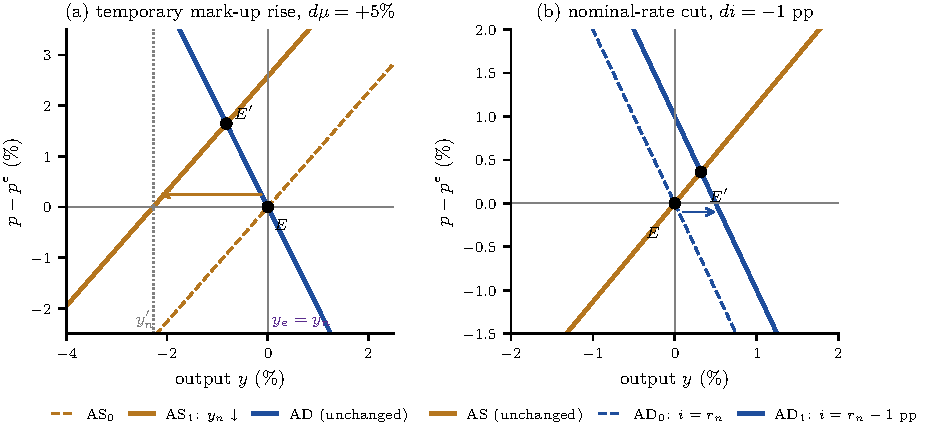
\includegraphics[width=\textwidth]{fig/fig_l7q2_shocks.pdf}
\caption{\small Question 2 in Benigno's calibration. (a) A temporary 5\% rise in the desired
mark-up: AS shifts up and to the left through $(p^e,y_n')$; AD does not move. (b) A
one-point cut in $i$: AD shifts up by one point (right by $\sigma=0.5$ points); AS does not
move. Interactive version: \href{\urlshocks}{\emph{Two Shocks}}.}
\label{fig:q2}
\end{figure}

%----------------------------------------------------------------------
\subsection*{Item (a) --- a temporary increase in firms' desired mark-ups}
%----------------------------------------------------------------------

\passo{Which curve shifts, and which way.}
A higher desired mark-up means a higher $\mu$ in eq.\ (13), whether it comes from more
monopoly power ($\theta\downarrow$), higher $\tau_w,\tau_y,\tau_l$, or a costlier
inelastically-demanded input such as oil (p.~513). By eq.\ (15):
\[
dy_n=-\frac{d\mu}{\sigma^{-1}+\eta}<0,\qquad dy_e=0 .
\]
\resp{AS shifts up and to the left}, through $(p^e,y_n')$ with $y_n'<y_n$. The vertical shift
at a given output is
\[
dp\big|_{y}=-\kappa\,dy_n=\frac{1-\alpha}{\alpha}\,d\mu .
\]
The $(1-\alpha)/\alpha$ factor is worth reading. The adjusting firms raise their price
\emph{relative to the index} by $d\mu$, and the index rises with them.

\resp{AD does not shift.} The shock is \emph{temporary}, so $\bar\mu$ and hence $\ybn$ are
unchanged, and $\mu$ does not appear in eq.\ (21). (A \emph{permanent} rise would also move
AD down through $\ybn$; that is a different question.)

\passo{Effects on output and prices.}
With $i$ unchanged at $\rho$, and since $r_n$ rises by $-dy_n/\sigma$, eq.\ \eqref{eq:closed}
gives
\[
dy=\frac{\sigma\kappa}{1+\sigma\kappa}\,dy_n<0,\qquad
dp=-\frac{\kappa}{1+\sigma\kappa}\,dy_n>0 .
\]
\resp{Output falls and the price level rises: stagflation.} With $d\mu=+5\%$:
$dy_n=-2.27\%$, $dy=-0.82\%$, $dp=+1.64\%$.

\passo{The two gaps have opposite signs.}
\[
y-y_n=-\frac{dy_n}{1+\sigma\kappa}=+1.45\%>0,\qquad y-y_e=dy=-0.82\%<0 .
\]
Output is \emph{above} the new natural level, which is why prices are rising: by AS, prices
move only with $y-y_n$. At the same time it is \emph{below} the efficient level, which is why
welfare has fallen.

\intuicao{The adjusting firms want a larger margin over marginal cost, so at any output they
charge more; that is the upward shift of AS. The price level rises. With $\pbar$ anchored,
a higher $p$ means lower expected inflation $\pbar-p$ and so a higher real rate
$i-(\pbar-p)$. Households save more and bring consumption down. Demand, and with it output,
falls along the unchanged AD curve. Output does not fall all the way to $y_n'$. The firms
with frozen prices keep selling at $p^e$, and as output falls, marginal cost falls with it,
which restrains the adjusting firms. The equilibrium $E'$ splits the shock between prices
and quantities in the ratio set by $\sigma\kappa$.}

\intuicao{Policy relevance, previewing Question 4. No interest rate restores both
targets. Holding $p=p^e$ requires \emph{raising} $i$ to $r_n$ (to 6.55\% here) and pushes
output down to $y_n'$. Holding $y=y_e$ requires \emph{cutting} $i$ and accepts a price rise
of $2.58\%$. Because $\mu$ moved $y_n$ without moving $y_e$, this is the model's genuine
trade-off.}

%----------------------------------------------------------------------
\subsection*{Item (b) --- a reduction in the nominal interest rate by the central bank}
%----------------------------------------------------------------------

\passo{Which curve shifts, and which way.}
$i$ appears only in AD. Solving eq.\ (21) for $p$,
\[
p=\pbar+\rho-i+\frac{\ybn-y}{\sigma},
\]
so a cut $di<0$ shifts \resp{AD up by $|di|$ at every output, equivalently to the right by
$\sigma|di|$}. \resp{AS does not move}: $y_n$ depends on $a$, $g$ and $\mu$, none of which
the central bank touches, and $p^e$ is predetermined.

\passo{Effects on output and prices.}
From eq.\ \eqref{eq:closed}, with $r_n$ unchanged:
\[
dy=-\frac{\sigma}{1+\sigma\kappa}\,di>0,\qquad dp=\kappa\,dy>0 .
\]
\resp{Output and the price level both rise}, moving up along AS. With $di=-1$ pp:
$dy=+0.32\%$, $dp=+0.36\%$. Since neither $y_n$ nor $y_e$ moved, both gaps equal $+0.32\%$.
Starting from $i=r_n$, the cut \emph{overheats} the economy: output rises above both its
natural and its efficient level.

\intuicao{At a given $p$, and with $\pbar$ anchored, a lower nominal rate is a lower
\emph{real} rate. Households substitute toward consumption today (the Euler equation), so
demand rises at every price level. The firms with frozen prices ($\alpha$) serve that demand
at $p^e$, so output rises. Hiring more labour raises the real wage households require, and
with it real marginal cost, so the $1-\alpha$ adjusting firms raise their prices. The price
level rises, which partly offsets the fall in the real rate. That feedback is why the
output response $\sigma/(1+\sigma\kappa)$ is smaller than the horizontal shift of AD,
$\sigma$.}

\intuicao{What does not happen. There is no liquidity effect through a money market and no
LM curve: the central bank sets $i$ directly. And the effect is purely short run. In the
second period every firm resets, $\bar y=\ybn$, and only $\pbar$ could be affected: money is
neutral in the long run (Benigno \S4.2). A cut is the right policy only when $r_n$ has
fallen, for example after a temporary productivity gain (\S6.1) or a fall in $\ybn$. In that
case it restores $E$ instead of overheating.}

\begin{tcolorbox}[trapbox, title={Traps in Question 2}]
\small
\begin{itemize}
\item \textbf{Shifting AD in (a).} A \emph{temporary} mark-up shock leaves $\ybn$ unchanged;
      only AS moves. The fall in demand is a movement \emph{along} AD caused by the higher
      price level.
\item \textbf{Reporting one ``output gap''.} After (a), $y-y_n>0$ while $y-y_e<0$. The first
      explains inflation, the second welfare.
\item \textbf{More rigidity makes AS steeper.} It is the opposite: $\alpha\uparrow\Rightarrow
      \kappa\downarrow$, flatter AS, and a rate cut moves output more and prices less.
\item \textbf{Using the IS--LM mechanism in (b)} (money supply up, liquidity effect). There
      is no LM curve; the channel is the real rate in the Euler equation.
\end{itemize}
\end{tcolorbox}

\begin{tcolorbox}[rubricbox]
\small
1.5 points per item. For each item the marks are for:
\begin{itemize}
\item the correct curve and direction (and, in (a), saying that AD does \emph{not} move);
\item the signs of $dy$ and $dp$;
\item the transmission mechanism in words (mark-up $\to$ prices $\to$ real rate $\to$
      demand; or rate $\to$ real rate $\to$ demand $\to$ marginal cost $\to$ prices).
\end{itemize}
Distinguishing the two gaps in (a) is what separates full marks from most answers.
\end{tcolorbox}

%======================================================================
\section{Question 3 \quad Natural versus efficient output}
%======================================================================

\passo{Definitions.}
\begin{itemize}
\item \textbf{Natural output $y_n$}: the output of the \emph{decentralised} economy when
      \emph{every} firm can reset its price. It is the flexible-price equilibrium of an
      economy that still has monopolistic competition and distortionary taxes. It is the
      anchor of AS, and $y-y_n$ drives \emph{prices}.
\item \textbf{Efficient output $y_e$}: the output a \emph{benevolent planner} would choose,
      maximising $u(C)-v(L)$ subject to $Y=C+G$ and $Y=AL$. It is the target in the
      welfare loss, and $y-y_e$ drives \emph{welfare}.
\end{itemize}
Neither concept involves price stickiness: $\alpha$ appears in neither. Stickiness explains
why $y$ differs from $y_n$. The mark-up explains why $y_n$ differs from $y_e$.

\passo{Step 1. The planner's condition.}
Substituting both constraints, the planner solves $\max_Y\,u(Y-G)-v(Y/A)$. The first-order
condition is
\[
\frac{v_l(Y_e/A)}{u_c(Y_e-G)}=A:\qquad \MRS=\MRT .
\]
The marginal rate of substitution between leisure and consumption equals the marginal rate of
transformation, which is labour productivity.

\passo{Step 2. The market's condition.}
With flexible prices every firm sets $P=(1+\mu)W/A$, so the real wage is $W/P=A/(1+\mu)$.
The household equates its $\MRS$ to that real wage (eq.\ 14):
\[
\frac{v_l(Y_n/A)}{u_c(Y_n-G)}=\frac{A}{1+\mu}.
\]
The two conditions are identical except for the wedge $1+\mu$.

\passo{Step 3. Log-linearise and subtract.}
With $v_l=L^\eta$, $u_c=C^{-\tilde\sigma^{-1}}$ and $\tilde\sigma^{-1}c=\sigma^{-1}(y-g)$, the
log of the $\MRS$ is $\eta(y-a)+\sigma^{-1}(y-g)$. The planner sets it equal to $a$, the
market to $a-\mu$. This gives eqs.\ (19) and (15), and
\[
\boxed{\;y_n-y_e=-\frac{\mu}{\sigma^{-1}+\eta}\;}
\]
(Benigno \S4.4, p.~509).

\passo{Why they differ under monopolistic competition.}
\resp{Market power drives a wedge between the marginal product of labour and the real wage.}
A firm facing downward-sloping demand restricts output to keep its price above marginal
cost. Equivalently, it pays labour only $A/(1+\mu)$ of what labour produces. The household
works until its $\MRS$ equals the wage it is paid, not the product it creates. So it works,
and the economy produces, \emph{too little}. At $y_n$ the value to society of one more unit
of output ($\MRT=A$) exceeds its cost to the household ($\MRS=A/(1+\mu)$), and an extra unit
would raise welfare. The shaded triangle in Figure~\ref{fig:q3}(i) is that lost surplus. Its
area grows with the square of the distance, $\tfrac12\Sg(y_n-y_e)^2$, which is why the
welfare loss is quadratic in $y-y_e$. Taxes act the same way, since every tax in eq.\ (13)
is part of $\mu$. In a perfectly competitive, tax-free economy ($\theta\to\infty$, all
$\tau=0$), $\mu=0$ and the two concepts coincide.

\begin{figure}[h]
\centering
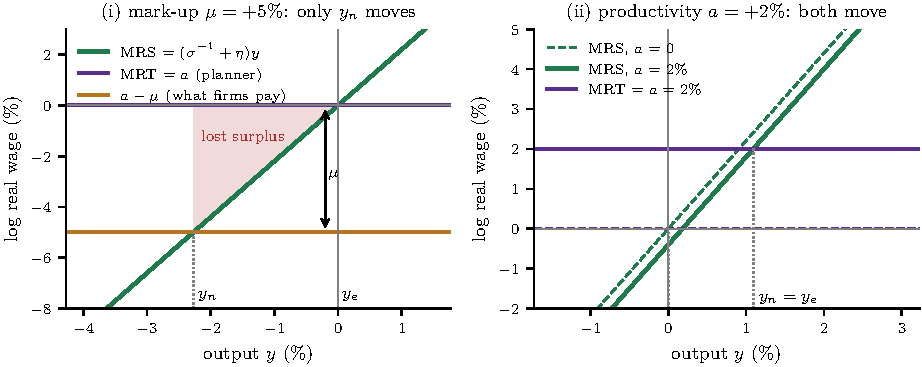
\includegraphics[width=\textwidth]{fig/fig_l7q3_wedge.pdf}
\caption{\small Question 3 in logs, Benigno's calibration ($\sigma^{-1}+\eta=2.2$).
(i) A 5\% mark-up lowers the wage firms pay, not the product of labour. The market stops at
$y_n=-2.27\%$ and the planner at $y_e=0$. (ii) A 2\% productivity gain raises both the $\MRT$
and the $\MRS$ curve's intercept, so $y_n$ and $y_e$ rise together to $1.09\%$.
Interactive version: \href{\urlwedge}{\emph{The Wedge}}.}
\label{fig:q3}
\end{figure}

\passo{Why a temporary rise in the desired mark-up changes $y_n$ but not $y_e$.}
Look at what enters each problem:
\[
y_n=y_n(a,\,g,\,\mu),\qquad y_e=y_e(a,\,g).
\]
The planner's problem contains \textbf{preferences, technology and resources} ($u$, $v$, $A$,
$G$) and nothing else. It contains no prices, no market power and no taxes. A mark-up is not
a change in what the economy \emph{can} produce or what households \emph{want}. It is a
change in how the \emph{market} allocates: a larger wedge between price and marginal cost.
So
\[
dy_n=-\frac{d\mu}{\sigma^{-1}+\eta}<0,\qquad dy_e=0 .
\]
\resp{The mark-up is an inefficient shock: it moves the economy's flexible-price outcome
without moving its welfare target.} ``Temporary'' adds only that $\bar\mu$, and hence
$\ybn$ and AD, stay put; $y_e$ would not move at any horizon.

Compare a productivity shock, Figure~\ref{fig:q3}(ii). It moves $\MRT$ and $\MRS$ by the same
amount in both problems, so $dy_n=dy_e$. That is an \emph{efficient} shock. The distinction
is the whole of Benigno's policy analysis:
\[
\text{a policy trade-off exists}\iff\text{the shock moves }y_n-y_e\iff\text{the shock moves }\mu .
\]

\intuicao{Why the distinction matters for policy. Monetary policy can close $y-y_n$, and by
doing so stabilise prices. When $y_n=y_e$ that also closes the welfare gap: the ``divine
coincidence'' of Benigno \S6. After a mark-up shock the two targets separate. Any interest
rate trades one against the other, and no interest rate can move $y_n$ back to $y_e$: that
would require removing the wedge itself, through tax cuts or competition policy.}

\begin{tcolorbox}[trapbox, title={Traps in Question 3}]
\small
\begin{itemize}
\item \textbf{``Natural'' $=$ ``optimal''.} $y_n$ is the flexible-price outcome of a
      \emph{distorted} economy. It is where prices are stable, not where welfare is highest.
\item \textbf{Attributing $y_n\neq y_e$ to sticky prices.} Neither concept depends on
      $\alpha$. The gap comes from market power and taxes alone.
\item \textbf{Saying the mark-up lowers $y_e$ because ``firms produce less''.} Firms do
      produce less, and that is $y_n$ falling. The planner's optimum has not moved, which is
      exactly why the fall is a welfare loss.
\end{itemize}
\end{tcolorbox}

\begin{tcolorbox}[rubricbox]
\small
2 points. The marks are for:
\begin{itemize}
\item the two definitions (flexible-price decentralised outcome versus planner's optimum);
\item the wedge argument ($\MRS=A/(1+\mu)$ against $\MRS=A$), ideally with
      $y_n-y_e=-\mu/(\sigma^{-1}+\eta)$;
\item the reason $\mu$ is absent from the planner's problem.
\end{itemize}
A contrast with a productivity shock is the cleanest way to show the last point.
\end{tcolorbox}

%======================================================================
\section{Question 4 \quad The loss function and the AS constraint}
%======================================================================

\begin{tcolorbox}[planbox, title={Map to Benigno's notation}]
\small
The question's loss is a general version of Benigno's eq.\ (33). Setting
\[
\phi_y=\tfrac12,\qquad \phi_p=\frac{\theta}{2\kappa},\qquad y^\ast=y_e
\]
recovers (33) exactly; setting $\phi_p=\phi/(2\kappa)$ with a free $\phi$ recovers the
mandate version (35). Everything below is solved for general $(\phi_y,\phi_p,y^\ast)$ and
then specialised.
\end{tcolorbox}

%----------------------------------------------------------------------
\subsection*{The shape of the loss function, and what it says about the central bank}
%----------------------------------------------------------------------

\[
\mathcal L=\phi_y\,(y-y^\ast)^2+\phi_p\,(p-p^e)^2,\qquad \phi_y,\phi_p>0 .
\]
\begin{enumerate}[label=\arabic*.]
\item \textbf{A bliss point.} The loss is zero only at $(y,p)=(y^\ast,p^e)$. The bank has
      \emph{two} targets: output at $y^\ast$ and no price surprise.
\item \textbf{Quadratic, so convex and symmetric.} Deviations in either direction are
      equally bad. A boom above $y^\ast$ is penalised as much as a recession below it, and
      a price rise as much as a fall. The bank is not trying to push output up; it
      \emph{stabilises} around a target. Convexity means the marginal loss rises with the
      size of the deviation: small misses are cheap and large ones very costly. So when the
      two targets conflict, the bank \emph{spreads} the miss across both instead of hitting
      one exactly and ignoring the other.
\item \textbf{Iso-loss curves are ellipses} centred at the bliss point
      (Figure~\ref{fig:q4}(i)). Their axis ratio is $\sqrt{\phi_y/\phi_p}$. A large
      $\phi_p/\phi_y$ gives flat, wide ellipses: the bank tolerates output deviations far
      more than price surprises.
\item \textbf{The relative weight $\phi_p/\phi_y$ is the bank's conservatism.} A large value
      is a hawk, a small one a dove. In the welfare-based version,
      $\phi_p/\phi_y=\theta/\kappa$, so the household \emph{itself} wants more weight on
      prices when goods are more substitutable ($\theta\uparrow$) or prices more rigid
      ($\alpha\uparrow\Rightarrow\kappa\downarrow$). The reason is that each price surprise
      then creates more costly relative-price dispersion (Benigno p.~522).
\item \textbf{The price term is $p-p^e$, not $p$.} Only \emph{unanticipated} movements are
      costly, because only they create dispersion between the firms that adjusted and those
      stuck at $p^e$. An anticipated price level is costless in this model.
\item \textbf{The output term uses $y^\ast$.} In the welfare-based loss $y^\ast=y_e$, not
      $y_n$. The bank cares about the allocation households experience, not about firms'
      marginal cost.
\end{enumerate}

%----------------------------------------------------------------------
\subsection*{Why the problem is subject to the AS condition}
%----------------------------------------------------------------------

The bank has \textbf{one instrument}, $i$, and it appears only in AD. Moving $i$ slides AD
along the AS curve, so the bank can reach \emph{any} point on AS, and \emph{only} points on
AS. The AS curve is private-sector behaviour that policy cannot override within the period.
The $1-\alpha$ adjusting firms price off marginal cost, the $\alpha$ others are stuck at
$p^e$, and $p^e$ was set before the shock.

So AS is the central bank's \emph{feasible set}. It is its opportunity frontier, exactly as a
budget line is a consumer's. AD is not a constraint: it contains the free variable $i$, so
for any point on AS there is an $i$ that puts AD through it. Choosing $(y,p)$ subject to AS
and then backing out $i$ is the same as choosing $i$ directly.

\passo{Solving it.}
The Lagrangian is
\[
\Lambda=\phi_y(y-y^\ast)^2+\phi_p(p-p^e)^2+\lambda\left[p-p^e-\kappa(y-y_n)\right].
\]
Its first-order conditions are
\[
2\phi_y(y-y^\ast)-\lambda\kappa=0,\qquad 2\phi_p(p-p^e)+\lambda=0 .
\]
Eliminating $\lambda$ gives the \textbf{targeting rule}:
\begin{equation}
\boxed{\;\phi_y\,(y-y^\ast)+\kappa\,\phi_p\,(p-p^e)=0\;}
\label{eq:rule}
\end{equation}
Geometrically, \eqref{eq:rule} is the tangency of an iso-loss ellipse with AS. The marginal
rate of substitution between the targets, $-\phi_y(y-y^\ast)/[\phi_p(p-p^e)]$, equals the
marginal rate of transformation $\kappa$ along AS. With Benigno's weights it becomes
$(y-y_e)+\theta(p-p^e)=0$, his eq.\ (34), the IT line.

Substituting AS into \eqref{eq:rule} gives
\begin{equation}
y^{o}=\frac{\phi_y\,y^\ast+\phi_p\kappa^2\,y_n}{\phi_y+\phi_p\kappa^2},\qquad
p^{o}-p^e=\frac{\kappa\,\phi_y}{\phi_y+\phi_p\kappa^2}\,(y^\ast-y_n),\qquad
\mathcal L^{o}=\frac{\phi_y\phi_p\kappa^2}{\phi_y+\phi_p\kappa^2}\,(y^\ast-y_n)^2 .
\label{eq:opt}
\end{equation}
Optimal output is a \emph{weighted average} of the target $y^\ast$ and the natural level
$y_n$. Everything hinges on one number, $y^\ast-y_n$: the distance between where the bank
wants output and where the AS curve crosses $p=p^e$. The bank implements $y^o$ with the
rate that puts AD through it. From eq.\ \eqref{eq:closed},
$i^o=r_n-(1+\sigma\kappa)(y^o-y_n)/\sigma$.

\begin{figure}[h]
\centering
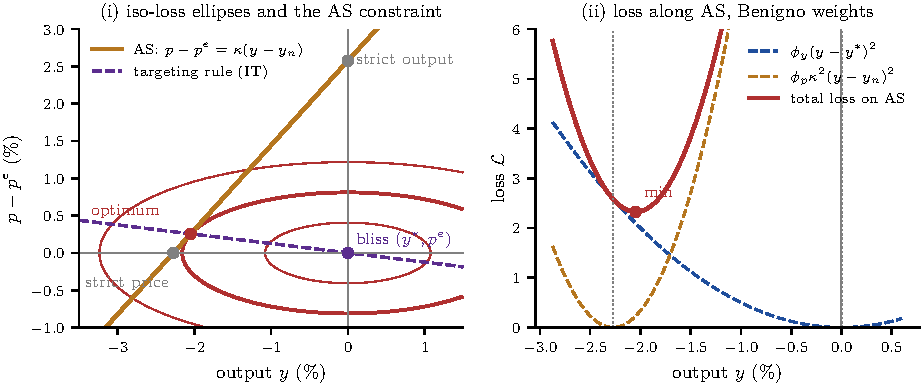
\includegraphics[width=\textwidth]{fig/fig_l7q4_loss.pdf}
\caption{\small Question 4 after a 5\% mark-up shock, with Benigno's weights ($\phi_y=\tfrac12$,
$\phi_p=\theta/2\kappa=3.53$, $y^\ast=y_e=0$). (i) The optimum is where an iso-loss ellipse
is tangent to AS. It lies on the targeting rule, between strict price stability and strict
output stabilisation. (ii) The same problem along AS: the output part falls and the price
part rises as $y$ moves from $y_n$ toward $y^\ast$, and the total is minimised in between.
Interactive version: \href{\urlloss}{\emph{The Loss Bowl}}.}
\label{fig:q4}
\end{figure}

%----------------------------------------------------------------------
\subsection*{What the AS constraint means for economic policy}
%----------------------------------------------------------------------

\passo{1. When $y^\ast=y_n$, the constraint does not bind: the divine coincidence.}
If the shock moves $y_n$ and $y^\ast=y_e$ together, as productivity and public spending do,
then AS passes through the bliss point. Eq.\ \eqref{eq:opt} gives $y^o=y^\ast$, $p^o=p^e$ and
$\mathcal L^o=0$. \resp{Stabilising prices and stabilising the welfare-relevant gap are the
same policy}, and the bank sets $i=r_n$.

\passo{2. When $y^\ast\neq y_n$, the constraint binds: a genuine trade-off.}
After a mark-up shock $y_n$ falls and $y_e$ does not, so AS misses the bliss point and
$\mathcal L^o>0$. With Benigno's weights and $y^\ast=y_e$, the optimum is
\[
p^o-p^e=\frac{1}{1+\theta\kappa}\cdot\frac{d\mu}{\sigma^{-1}+\eta},\qquad
y^o-y_e=-\frac{\theta\kappa}{1+\theta\kappa}\cdot\frac{d\mu}{\sigma^{-1}+\eta}.
\]
\resp{The bank lets a fraction $1/(1+\theta\kappa)$ of the shock into prices and absorbs the
rest as an output loss.} With $\theta\kappa=9.07$ that fraction is $9.9\%$. For
$d\mu=+5\%$: $y^o=-2.05\%$ and $p^o-p^e=+0.26\%$. The implementing rate is
$i^o=5.84\%$: a rise from $2\%$, but less than the $6.55\%$ ($=r_n$) that strict price
stability would need. The two limits are the corners of Figure~\ref{fig:q4}(i):
$\phi_p/\phi_y\to\infty$ is strict price stability ($y=y_n$, $p=p^e$);
$\phi_p/\phi_y\to0$ is strict output stabilisation ($y=y^\ast$, $p-p^e=2.58\%$). Even the
\emph{sign} of the response relative to doing nothing depends on the mandate (p.~522). A
bank less concerned with prices, whose IT line is steeper than AD, would \emph{cut} rates
after the same shock.

\passo{3. Monetary policy chooses a point on AS; it cannot move AS.}
The constraint encodes what the central bank \emph{cannot} do. It cannot change $y_n$, so it
cannot close $y_n-y_e$. The permanent part of that gap, the level distortion from market
power and taxes, is a job for \emph{structural and fiscal} policy: a subsidy or a cut in
$\tau_w$, $\tau_l$ or $\tau_y$ that lowers $\mu$, or competition policy that raises $\theta$.
Asking monetary policy to deliver $y^\ast>y_n$ \emph{permanently} is asking it to beat a
constraint it does not control.

\passo{4. The trade-off exists only because prices are sticky, and only in the short run.}
The slope of the frontier is $\kappa$. As $\alpha\to0$, $\kappa\to\infty$ and AS becomes
vertical at $y_n$: the bank can choose $p$ but not $y$, and the optimum is $p=p^e$. In the
second period every firm resets, AS is vertical, and policy only sets $\pbar$. Moreover $p^e$
is predetermined \emph{within} the period, not forever. If the bank tried to hold $y$ above
$y_n$ every period, price-setters would build that into $p^e$. Surprises cannot be
systematic: with rationally set $p^e$ they average zero, so $y=y_n$ on average whatever the
bank wants. This is the time-inconsistency logic of Kydland--Prescott and Barro--Gordon, and
it is why Benigno approximates welfare around an \emph{efficient} steady state
(fn.~21, p.~522). There $y_n=y_e$ absent shocks, so the bank has no permanent incentive to
surprise.

\passo{5. A rule the bank can follow without knowing the shock.}
Eq.\ \eqref{eq:rule} does not mention the shock. A bank that keeps
$\phi_y(y-y^\ast)+\kappa\phi_p(p-p^e)=0$ responds optimally to productivity, spending and
mark-up shocks, whether temporary, permanent or expected. This is Benigno's argument
(pp.~521--522, after Giannoni and Woodford, 2002) for a \emph{targeting rule} over a Taylor
rule, whose optimal coefficients depend on the shock process. It is also what ``flexible
inflation targeting'' means operationally (Svensson): let prices deviate only in proportion
to the output sacrifice the AS curve would otherwise force.

\begin{tcolorbox}[trapbox, title={Traps in Question 4}]
\small
\begin{itemize}
\item \textbf{Using AD as the constraint.} AD contains the instrument, so it restricts
      nothing. AS is the constraint because it is the one relation policy cannot shift.
\item \textbf{Setting $y^\ast=y_n$ in the welfare-based loss.} The welfare target is $y_e$.
      With $y^\ast=y_n$ there is never a trade-off, and the question loses its point.
\item \textbf{``The bank minimises inflation.''} It minimises price \emph{surprises}
      $p-p^e$, jointly with output deviations. The weights decide how the unavoidable miss
      is split.
\item \textbf{Reading $\kappa$ as a policy choice.} It is the private sector's pricing
      technology. The bank takes it as given, exactly as a consumer takes prices as given.
\end{itemize}
\end{tcolorbox}

\begin{tcolorbox}[rubricbox]
\small
2 points. The marks are for:
\begin{itemize}
\item the shape: bliss point, convexity and symmetry, and the relative weight as the
      bank's conservatism;
\item the reason AS is the constraint (one instrument, which moves AD only; AS is the
      feasible set);
\item the policy meaning: no trade-off when $y^\ast=y_n$, a trade-off after mark-up shocks,
      and monetary policy's inability to move $y_n$.
\end{itemize}
The targeting rule \eqref{eq:rule} and the split $1/(1+\theta\kappa)$ are the full-marks
extension.
\end{tcolorbox}

\vspace{6pt}
\begin{center}
\small\color{gray}
Figures: \texttt{Resolucao/lista7\_codigo/l7\_figuras.py}. Derivations:
\texttt{Map/benigno/} notes 02, 03, 04, 06, 10. Routing note: \texttt{Map/lista-07.md}.
\end{center}

\end{document}
